\documentclass[tikz,border=10pt]{standalone}
\usepackage{tikz}
\usetikzlibrary{arrows.meta}

\tikzset{
  sfgsource/.style={circle, draw=green!60!black, line width=1.2pt, minimum size=1.0cm, inner sep=0pt},
  sfgnode/.style={circle, draw=purple!70!black, line width=1.2pt, minimum size=1.0cm, inner sep=0pt},
  sfgsink/.style={circle, draw=red!70!black, line width=1.2pt, minimum size=1.0cm, inner sep=0pt},
  sfgedge/.style={->, line width=1.2pt, draw=black!80, >=Stealth},
  gain/.style={font=\small\itshape, fill=white, inner sep=1pt}
}

\begin{document}
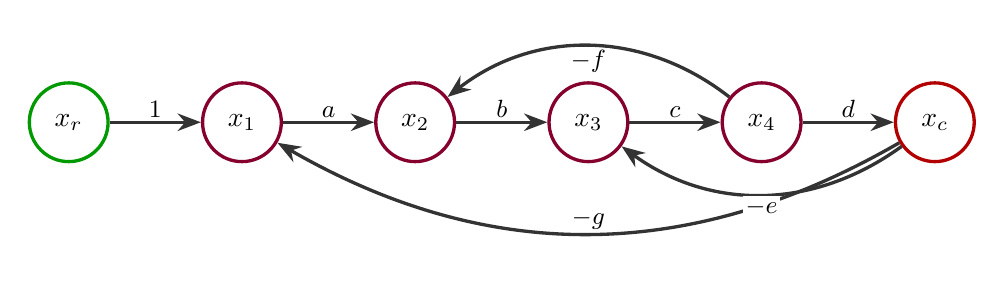
\begin{tikzpicture}
  \node[sfgsource] (xr) at (0,0) {$x_r$};
  \node[sfgnode] (x1) at (2.2,0) {$x_1$};
  \node[sfgnode] (x2) at (4.4,0) {$x_2$};
  \node[sfgnode] (x3) at (6.6,0) {$x_3$};
  \node[sfgnode] (x4) at (8.8,0) {$x_4$};
  \node[sfgsink] (xc) at (11.0,0) {$x_c$};

  \draw[sfgedge] (xr) -- node[gain, above] {$1$} (x1);
  \draw[sfgedge] (x1) -- node[gain, above] {$a$} (x2);
  \draw[sfgedge] (x2) -- node[gain, above] {$b$} (x3);
  \draw[sfgedge] (x3) -- node[gain, above] {$c$} (x4);
  \draw[sfgedge] (x4) -- node[gain, above] {$d$} (xc);

  \draw[sfgedge, bend left=30] (xc) to node[gain, above] {$-g$} (x1);
  \draw[sfgedge, bend left=36] (xc) to node[gain, below] {$-e$} (x3);
  \draw[sfgedge, bend right=38] (x4) to node[gain, below] {$-f$} (x2);
\end{tikzpicture}
\end{document}
